% team_and_abstract.tex
\textbf{Team Members:}

\begin{figure}[htbp]
    \centering
    \begin{minipage}[t]{0.2\textwidth}
        \centering
        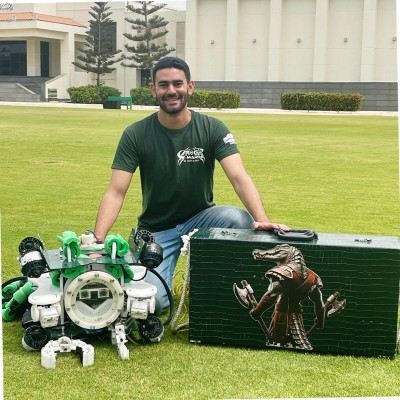
\includegraphics[width=\textwidth]{figs/ahmed.png}
    \end{minipage}
    \hfill
    \begin{minipage}[t]{0.2\textwidth}
        \centering
        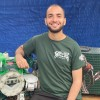
\includegraphics[width=\textwidth]{figs/fares.png}
    \end{minipage}
    \hfill
    \begin{minipage}[t]{0.2\textwidth}
        \centering
        
\includegraphics[width=\textwidth]{figs/dawood.png}
    \end{minipage}
    \hfill
    \begin{minipage}[t]{0.2\textwidth}
        \centering
        
\includegraphics[width=\textwidth]{figs/omar.png}
    \end{minipage}
    \hfill
    \begin{minipage}[t]{0.2\textwidth}
        \centering
        
\includegraphics[width=\textwidth]{figs/yousri.png}
    \end{minipage}
    \hfill
    \begin{minipage}[t]{0.2\textwidth}
        \centering
        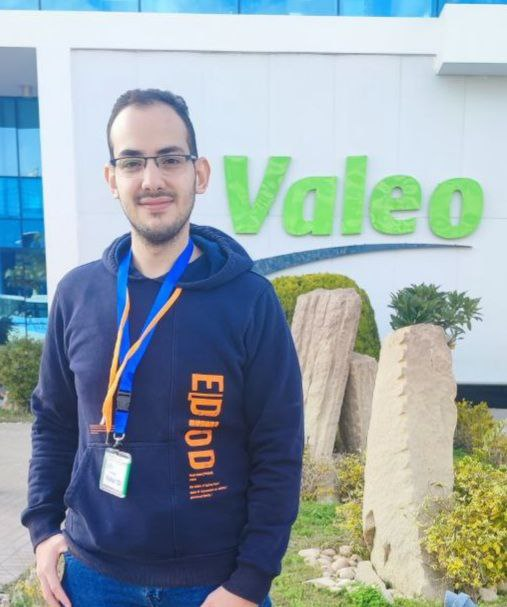
\includegraphics[width=\textwidth]{figs/ashraf.png}
    \end{minipage}
\end{figure}

\vspace{3cm}

\begin{center} % Centering the abstract
\begin{abstract}
    \Large % Adjust the font size here (e.g., \Large, \huge, etc.)
    In this paper, we present a smart home IoT project that utilizes an ESP32 microcontroller and a mobile application for remote control and monitoring. The system allows users to access and control various aspects of their home, including doors, windows, and active systems, from anywhere with an internet connection. We discuss the components, architecture, and functionality of the project, highlighting its potential benefits and applications.
\end{abstract}
\end{center}
